\documentclass{controle}
\usepackage{main}

\title{Contrôle n°1 : Fonctions polynomiales du second degré, Taux de variation}
\date{6 Octobre 2025}
\author{Première Spécialité Mathématiques}

\begin{document}
\maketitle

\instructions[Interdite]

\begin{questions}
\titledquestion{Taux de variation}[4]
Soit $f$ une fonction, et $a < b$ deux réels. Dans chacun des cas suivants, calculer le taux de variation de $f$ entre $a$ et $b$. De plus, justifier ce qui aurait pu être obtenu sans calcul dans votre résultat.
\begin{parts}
\part $f \colon x \mapsto 7x - 1$; $a = 9$ et $b = 11$
\part $f \colon x \mapsto 5(x - 8)^2 + 9$; $a = 2$ et $b = 4$
\part $f \colon x \mapsto -(x + 4)^2 -2$; $a = -5$ et $b = -1$
\part $f \colon x \mapsto 1 - 3x$; $a = 0$ et $b = 8$
\end{parts}
\vspace*{1cm}
\titledquestion{Étude de fonctions polynomiales du second degré}[4]
Pour chacune des fonctions polynomiales du second degré ci-dessous, dresser le tableau de variations de cette fonction.
\begin{parts}
\part $f \mapsto x^2 + 2x$
\part $g \mapsto 2x^2 - 20x + 54$
\part $u \mapsto -5x^2 -30x - 48$
\part $v \mapsto -3x^2 - 1$
\end{parts}
\vspace*{1cm}
\titledquestion{Arc-en-ciel}[6]
L'entrée d'un édifice ancien utilise une arche pour accueillir ses visiteurs. Un géomètre est chargé d'en mesurer la hauteur. Il commence alors par mesurer la longueur au sol de cette arche : \qty{4}{\meter}. Il constate aussi qu'en s'éloignant du bord gauche de \qty{1}{\meter}, sa tête touche l'arche. Il mesure \qty{2}{\meter}.

On suppose que l'arche peut-être représenté à l'aide d'une parabole d'équation $y = ax^2 + bx + c$, où $x$ représente la distance au sol par rapport au bord gauche.

\begin{center}
\begin{tikzpicture}
\coordinate (BL) at (-0.25,-0.25);
\coordinate (TR) at (4.25,3.25);

\draw[help lines] (BL) grid[step=0.5] (TR);
\draw[axis] (BL |-,0) -- (TR |-,0) node[right] {$x$};
\draw[axis] (0, |- BL) -- (0, |- TR) node[above] {$y$};

\draw (4,0) node[below=0.3cm] {$4$};
\draw (0,0) node[below=0.3cm] {$0$};

\draw[dashed] (1,0) node[below] {$1$} -- (1,2) -- (0,2) node[left] {$2$};

\clip (BL) rectangle (TR);

\draw plot[samples=100] (\x, {-2/3*\x*\x + 8/3*\x});
\end{tikzpicture}
\end{center}
\begin{parts}
\part[1] Quel est le signe de $a$ ?
\part[1] À l'aide des informations données dans l'énoncé ou dans le schéma, déterminer la valeur de $c$.

On suppose que la forme canonique de ce polynôme du second degré se note $a(x - \alpha)^2 + \beta$.
\part[2] En utilisant un argument sur l'axe de symétrie de la parabole, en déduire la valeur de $\alpha$.
\part[2] On admet sans démonstration que le polynôme du second degré est aussi égal à sa forme factorisée $ax(x-4)$. En déduire la valeur de $a$, puis la valeur de $\beta$.
\end{parts}

\vspace*{1cm}
\titledquestion{Vous avez carte blanche}[6]
Soit $ABCD$ un rectangle tel que $AB = \qty{10}{\centi\meter}$ et $AD = \qty{6}{\centi\meter}$. 

On pose $E$ un point \textbf{mobile} du segment $[AB]$ et $G$ un point du segment $[AD]$ tel que $AE = AG$. On pose $F$ tel que $AEFG$ est un carré. 

On pose $I$ un point du segment $[BC]$ et $H$ un point du segment $[CD]$ tel que le quadrilatère $FICH$ est un rectangle. 

On pose $x = AE$. On s'intéresse à l'aire $M(x)$ de la \textbf{partie laissée blanche}, c'est-à-dire l'aire du triangle $AEF$ et l'aire du triangle $FHC$.
\begin{center}
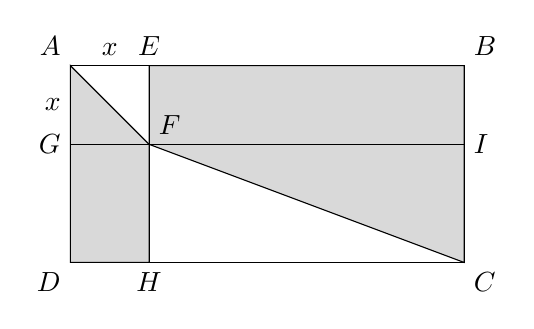
\begin{tikzpicture}
\coordinate (A) at (0,0);
\coordinate (B) at (5,0);
\coordinate (C) at (5,-2.5);
\coordinate (D) at (0,-2.5);

\coordinate (E) at (1,0);
\coordinate (G) at (0,-1);
\coordinate (F) at (1,-1);

\coordinate (I) at (5,-1);
\coordinate (H) at (1,-2.5);

\fill[color=gray!30] (A) -- (F) -- (H) -- (D) -- cycle;
\draw (A) -- (F) -- (H) -- (D) -- cycle;
\fill[color=gray!30] (E) -- (F) -- (C) -- (B) -- cycle;
\draw (E) -- (F) -- (C) -- (B) -- cycle;

\draw (A) -- (B) -- (C) -- (D) -- cycle;
\draw (A) -- (E) -- (F) -- (G) -- cycle;
\draw (F) -- (I) -- (C) -- (H) -- cycle;

\draw (A) node[above left] {$A$};
\draw (B) node[above right] {$B$};
\draw (C) node[below right] {$C$};
\draw (D) node[below left] {$D$};
\draw (E) node[above] {$E$};
\draw (G) node[left] {$G$};
\draw (F) node[above right] {$F$};
\draw (I) node[right] {$I$};
\draw (H) node[below] {$H$};

\draw (A) -- (G) node[midway,left] {$x$};
\draw (A) -- (E) node[midway,above] {$x$};
\end{tikzpicture}
\end{center}
\begin{parts}
\part[1] Justifier que $x$ est dans l'intervalle $[0;6]$.
\part[2] Démontrer alors que pour tout $x \in [0;6]$,
\begin{equation*}
M(x) = x^2 - 8x + 30  
\end{equation*}
\part[1] Tracer le tableau de variations de l'aire laissée blanche. 

En déduire la valeur de $x$ pour laquelle cette aire est minimale.
\part[2] Montrer que quelque soit la valeur de $x$, l'aire blanche est toujours supérieure à l'aire du rectangle $GFDH$. (Indication : Si on pose $N(x)$ l'aire de $GFDH$, on étudiera le signe $M(x) - N(x)$)  
\end{parts}
\end{questions}
\end{document}